\documentclass[dvipsnames, compress]{beamer}

\usepackage{currfile}
\usepackage{pgfpages}
% \setbeameroption{hide notes} % Only slides
% \setbeameroption{show only notes} % Only notes
% \setbeameroption{show notes on second screen=right} % Both
% \setbeamertemplate{note page}{\pagecolor{yellow!5}\insertnote}\usepackage{palatino}


%%%%%%%%%%%%%%%%%%%%%%%%%%%%%%%%%%%%%%%%%
% Beamer Presentation
% LaTeX Template
% Version 1.0 (10/11/12)
%
% This template has been downloaded from:
% http://www.LaTeXTemplates.com
%
% License:
% CC BY-NC-SA 3.0 (http://creativecommons.org/licenses/by-nc-sa/3.0/)
%
%%%%%%%%%%%%%%%%%%%%%%%%%%%%%%%%%%%%%%%%%

%----------------------------------------------------------------------------------------
%	PACKAGES AND THEMES
%----------------------------------------------------------------------------------------




\mode<presentation> {

% The Beamer class comes with a number of default slide themes
% which change the colors and layouts of slides. Below this is a list
% of all the themes, uncomment each in turn to see what they look like.
%\usetheme{default}
%\usetheme{AnnArbor}
%\usetheme{Antibes}
%\usetheme{Bergen}
%\usetheme{Berkeley}
%\usetheme{Berlin}
%\usetheme{Boadilla}
%\usetheme{CambridgeUS}
%\usetheme{Copenhagen}
%\usetheme{Darmstadt}
%\usetheme{Dresden}
%\usetheme{Frankfurt}
%\usetheme{Goettingen}
%\usetheme{Hannover}
%\usetheme{Ilmenau}
%\usetheme{JuanLesPins}
%\usetheme{Luebeck}
%\usetheme{Madrid}
%\usetheme{Malmoe}
%\usetheme{Marburg}
%\usetheme{Montpellier}
%\usetheme{PaloAlto}
%\usetheme{Pittsburgh}
%\usetheme{Rochester}
%\usetheme{Singapore}
%\usetheme{Szeged}
\usetheme{Warsaw}

% As well as themes, the Beamer class has a number of color themes
% for any slide theme. Uncomment each of these in turn to see how it
% changes the colors of your current slide theme.

%\usecolortheme{albatross}
%\usecolortheme{beaver}
%\usecolortheme{beetle}
%\usecolortheme{crane}
%\usecolortheme{dolphin}
%\usecolortheme{dove}
%\usecolortheme{fly}
%\usecolortheme{lily}
%\usecolortheme{orchid}
%\usecolortheme{rose}
%\usecolortheme{seagull}
%\usecolortheme{seahorse}
\usecolortheme{whale}
%\usecolortheme{wolverine}

%\setbeamertemplate{footline} % To remove the footer line in all slides uncomment this line
%\setbeamertemplate{footline}[frame number] % To replace the footer line in all slides with a simple slide count uncomment this line
\useoutertheme{miniframes}

%\setbeamertemplate{navigation symbols}{} % To remove the navigation symbols from the bottom of all slides uncomment this line

\setbeamercovered{transparent} % Fait apparaître les animations en grisé (utile pour la conception, mais peut être commenté lors de la remise du document final)

% Pour utiliser une police à empattements partout
\usefonttheme{serif}

% Pour rajouter la numérotation des frames dans les pieds de page
\newcommand*\oldmacro{}%
\let\oldmacro\insertshorttitle%
\renewcommand*\insertshorttitle{%
  \oldmacro\hfill%
  \insertframenumber\,/\,\inserttotalframenumber
  }
}

\beamertemplatenavigationsymbolsempty
\addtobeamertemplate{navigation symbols}{}{%
\usebeamerfont{footline}%
\usebeamercolor[fg]{footline}%
\hspace{1em}%
%\insertframenumber/\inserttotalframenumber
}

\usepackage{graphicx} % Allows including images
\usepackage{booktabs} % Allows the use of \toprule, \midrule and \bottomrule in tables
\setbeamercovered{invisible}

\usepackage{natbib}         % Pour la bibliographie
\usepackage{url}            % Pour citer les adresses web
\usepackage[T1]{fontenc}    % Encodage des accents
\usepackage[english]{babel}
\usepackage[utf8]{inputenc} % Lui aussi
\usepackage{numprint}       % Histoire que les chiffres soient bien

\usepackage{amsmath}        % La base pour les maths
\usepackage{mathtools}
\usepackage{mathrsfs}       % Quelques symboles supplémentaires
\usepackage{amssymb}        % encore des symboles.
\usepackage{amsfonts}       % Des fontes, eg pour \mathbb.
\usepackage{array}
\usepackage{cancel}
\usepackage{stackengine}    % text above other text
\usepackage{ifthen}         % ifthenelse

\usepackage{hyperref}


%%% Si jamais vous voulez changer de police: décommentez les trois
%\usepackage{tgpagella}
%\usepackage{tgadventor}
%\usepackage{inconsolata}

\usepackage{xcolor} % De la couleur
\usepackage{graphicx} % inclusion des graphiques
\usepackage{wrapfig}  % Dessins dans le texte.

\usepackage{listings} % Code blocks
\usepackage{rustlistings}

% \usepackage{tabulary} % 

\usepackage{tikz}     % Un package pour les dessins (utilisé pour l'environnement {code})
%\usepackage{tikz-cd}
\usetikzlibrary{automata,positioning,arrows,trees}
\usetikzlibrary{decorations.pathreplacing}
\usepackage{adjustbox}
\usepackage[framemethod=TikZ]{mdframed}

\usepackage{pifont} % extra symbols
\usepackage[normalem]{ulem} % strikeout
\usepackage{appendixnumberbeamer} % no numbering after last slide

% Ce fichier contient toutes les macros que vous pouvez avoir envie de définir
% si vous les utilisez plusieurs fois dans le document.

\PassOptionsToPackage{svgnames}{color}

% Un environnement pour bien présenter le code informatique
\newenvironment{code}{%
\begin{mdframed}[linecolor=green,innerrightmargin=30pt,innerleftmargin=30pt,
backgroundcolor=black!5,
skipabove=10pt,skipbelow=10pt,roundcorner=5pt,
splitbottomskip=6pt,splittopskip=12pt]
}{%
\end{mdframed}
}

\newcommand{\bijective}{%
  \hookrightarrow\mathrel{\mspace{-15mu}}\rightarrow
}
\newcommand{\surjective}{\twoheadrightarrow}
\newcommand{\injective}{\hookrightarrow}
\newcommand{\implication}{\Longrightarrow}
\newcommand{\impl}{\Rightarrow}
\newcommand{\reciprocal}{\Longleftarrow}
\newcommand{\equivalent}{\Longleftrightarrow}
\newcommand{\NN}{\ensuremath{\mathbb{N}}}
\newcommand{\RR}{\ensuremath{\mathbb{R}}}
\newcommand{\QQ}{\ensuremath{\mathbb{Q}}}
\newcommand{\ZZ}{\ensuremath{\mathbb{Z}}}
\newcommand{\CC}{\ensuremath{\mathbb{C}}}
\newcommand{\EE}{\ensuremath{\mathbb{E}}}
\newcommand{\PP}{\ensuremath{\mathbb{P}}}
\renewcommand{\epsilon}{\varepsilon}
\renewcommand{\phi}{\varphi}
\renewcommand{\leq}{\leqslant}
\renewcommand{\geq}{\geqslant}

\newcommand{\bbrack}[1]{\left\llbracket#1\right\rrbracket}

\newcommand{\inv}[1]{#1^{-1}}

\newcommand{\tsf}[1]{\textsf{#1}}
\newcommand{\ttt}[1]{\texttt{#1}}
\newcommand{\tbf}[1]{\textbf{#1}}
\newcommand{\tsc}[1]{\textsc{#1}}
\newcommand{\tq}{\ |\ }
\newcommand{\abs}[1]{\ensuremath{\left|#1\right|}}
\newcommand{\set}[1]{\ensuremath{\left\{#1\right\}}}
\newcommand{\paren}[1]{\ensuremath{\left(#1\right)}}

\newcommand\semantics{%
    \mathrel{\rightsquigarrow}}


\newlength{\mirageWidth}\newlength{\mirageHeight}
\newcommand{\mirage}[1]{% The opposite of a \phantom: it is visible but it takes no space
    #1%
    \settowidth{\mirageWidth}{#1}%
    \settoheight{\mirageHeight}{#1}%
    \hspace{-\mirageWidth}%
    \vspace{-\mirageHeight}%
}

\DeclareMathOperator{\poly}{poly}
\DeclareMathOperator{\expn}{exp}
\DeclareMathOperator{\minvolume}{\exists\textup{\tsf{MVol}}}
\DeclareMathOperator{\avgvolume}{\textup{\tsf{EMVol}}}
\DeclareMathOperator{\maxvolume}{\textup{\tsf{DMVol}}}
\DeclareMathOperator{\radius}{\textup{\tsf{MRad}}}
\newcommand{\neigh}{\mathcal{N}}

\newenvironment{stacked}{%
    \begin{tikzpicture}%
        \node (ref) {};%
}{%
    \end{tikzpicture}%
}

\newcommand{\stackitem}[2]{%
    \node at (ref) {{%
        \visible<#1>{%
            \begin{minipage}{\textwidth}
                #2%
            \end{minipage}
        }%
    }};%
}

\newcommand{\runnable}[2]{%
    \begin{block}{Demo}%
        \href{run:run/#1.sh}{\texttt{#2}}%
    \end{block}%
}

\newcommand{\cmark}{\color{darkgreen}{\ding{51}}} % check mark
\newcommand{\xmark}{\color{red}{\ding{55}}} % cross mark


\title[TreeBor]{Tree Borrows}
\subtitle{An aliasing model for Rust}
\author{Neven \textsc{Villani}}
\date{Oct 2022 - Jun 2023\\at MPI-SWS Saarbr\"ucken}

\renewcommand{\familydefault}{\sfdefault}
\begin{document}


% What structure do we want for the presentation ?
% In no particular order:
%[ ] - SB basics
%[X]   - quick word on 2-phase borrows
%[X]   - same interface
%[X]   - stack structure and comparison of dimensions
%[ ] - comparison with SB
%[ ]   - are the lost optimizations important ?
%[ ]     - spurious writes: can't assume termination
%[ ]   - what more code can we write ?
%[ ]     - copy_nonoverlapping is a good selling point
%[X] - derivation of the tree structure
%[X]   - with things that should not change anything significant
%[X]     - `fn(&x) { x }` ~ `fn(&x) { &*x }`
%[X]     - `*_ = 1` ~ `*(&*_) = 1`
%        showing that it is basically mandatory that we only
%        distinguish between child vs self vs foreign,
%        then the lack of distinction between child and self is a choice,
%        not a necessity.
%[X]   - some freedom in when we create a new pointer:
%        it's easy to define "equivalence classes" of "this reference
%        and all its raw copies"
%[X] - necessary rules
%[X]   - noalias requirements
%[X]   - unique path of Active
%[ ] - chosen rules
%[X]   - Active -> Frozen
%[X]   - everything starts Reserved
%[X]   - not writing on function entry
%[ ]   for each of these show what we would lose/gain in terms of patterns/optimizations
%      if we changed them.
%[X] - how to use / a working example
%[X]   - MIRIFLAGS
%[X]   - interpretation of errors

%\begin{frame}
    \titlepage
\end{frame}

\section{Introduction}

\begin{frame}[fragile,t]
    \frametitle{Why have UB?}
    \framesubtitle{A simple(r) example}

    \begin{lstlisting}[language=rust]
enum bool {
    true = 1,
    false = 0,
}
    \end{lstlisting}

    \begin{onlyenv}<2>
        What happens if...
        \begin{lstlisting}[language=rust]
let b: bool = 2;
        \end{lstlisting}
    \end{onlyenv}

    \begin{onlyenv}<3>
        What happens if...
        \begin{lstlisting}[language=rust]
let b: bool = unsafe { std::mem::transmute(2) };
//             ^^^^^^ remember this
let notb = !b; // ?
let notnotb = !notb;
assert!(b == notnotb); // ???
        \end{lstlisting}
        Can the compiler optimize a double negation into the identity ?
    \end{onlyenv}

    \begin{onlyenv}<4>
        What happens if...
        \begin{lstlisting}[language=rust, escapechar=@]
let b: bool = unsafe { std::mem::transmute(2) };
// UB: invalid value
@@
@@
@@
        \end{lstlisting}
        The compiler \textit{can} optimize a double negation into the identity.\\
        The compiler can do \textit{anything} once you have constructed an invalid value.
    \end{onlyenv}
\end{frame}

\begin{frame}[fragile]
    \frametitle{Rust's type system}
    \begin{onlyenv}<1>
        \begin{lstlisting}[language=rust]
let t: T = v;
//          ^ value
//      ^ type
//  ^ variable
//  ^^^^^^^^ variable binding

fn incr(n: u8) -> u8 {
    n + 1
}

fn main() {
    let n: u8 = 42;
    let m: u8 = incr(n);
    println!("{n} + 1 = {m}");
}
        \end{lstlisting}
    \end{onlyenv}

    \begin{onlyenv}<2>
        \begin{lstlisting}[language=rust]
// Primitives
f32, f64, u8, i8, u16, i16, u32, i32,
u64, i64, u128, i128, usize, isize, bool
// Products
struct Point {
    x: f64,
    y: f64,
}
type Triplet = (f64, f64, usize);
type Array = [f64; 10];
// Sums
enum Shape {
    Circle(Point, f64),
    Square(Point, f64),
    Triangle([Point; 3]),
}
        \end{lstlisting}
    \end{onlyenv}

    \begin{onlyenv}<3>
        \begin{lstlisting}[language=rust, escapechar=@]
// Smart pointers
Box<T>, Rc<T>, Arc<T>, Cow<T>

// Raw pointers
*const T
*mut T
// (*const T @\(\sqsubset\)@ *mut T)

// References
@@&'a T // shared and immutable
@@&'a mut T // unique and mutable
// (&'a T @\(\sqsubset\)@ &'a mut T)
// ('a @\(\subset\)@ 'b @\(\Rightarrow\)@ &'a T @\(\sqsubset\)@ &'b T)
// ('a @\(\subset\)@ 'b @\(\Rightarrow\)@ &'a mut T @\(\sqsubset\)@ &'b mut T)
        \end{lstlisting}
    \end{onlyenv}

    \begin{onlyenv}<4>
        Just like
        \begin{lstlisting}[language=rust]
// x: &mut bool
*x = 4;
        \end{lstlisting}
        is a type error (mismatched types \texttt{bool} and \texttt{u8}),
        \begin{lstlisting}[language=rust]
// x: &u8
*x = 4;
        \end{lstlisting}
        is also a type error (\texttt{\&\_} does not support assignment),
        and so is
        \begin{lstlisting}[language=rust]
// n: u8
let p = (&mut n, &mut n);
        \end{lstlisting}
        (impossible to satisfy lifetime constraints).\\

        Mutability and uniqueness are part of the type!\\
        Can we exploit that?
    \end{onlyenv}

\end{frame}

\begin{frame}[fragile,t]
    \frametitle{What is \texttt{unsafe}?}
    The type system of Rust is a bit too strict for some low-level applications.\\
    The \texttt{unsafe} keyword gives access to the language \textit{unsafe Rust},
    superset of Rust, where you can
    \begin{itemize}
        \item dereference raw pointers,
        \item call \texttt{unsafe} functions,
        \item do ffi.
    \end{itemize}

    This has the effect of making \texttt{unsafe} an escape hatch to locally bypass the type checker.
    \begin{exampleblock}{From the previous example}
        \texttt{std::mem::transmute} is an \texttt{unsafe} function, thus the
        use of \texttt{unsafe \{ std::mem::transmute(2) \}}.
    \end{exampleblock}
\end{frame}

\begin{frame}[fragile, t]
    \frametitle{A motivating example for Aliasing UB}
    \begin{lstlisting}[language=rust]
fn foo(x: &mut u64) {
    let val = *x;
    opaque();
    *x = val;
}
    \end{lstlisting}
    optimized into
    \begin{lstlisting}[language=rust]
fn foo(x: &mut u64) {
    opaque();
}
    \end{lstlisting}
    Well-typedness of any program that calls \texttt{foo} implies uniqueness
    of \texttt{x} during the execution of \texttt{foo}: \texttt{opaque} cannot mutate \texttt{x}!\\
    \begin{onlyenv}<2->
    ...except if the user uses \texttt{unsafe} to bypass the uniqueness check\\
    \end{onlyenv}
    \begin{onlyenv}<3>
    ...which we are going to assume does not happen: we will declare it to be UB
    to use \texttt{unsafe} to violate the requirement of uniqueness on mutable references.
    \end{onlyenv}
\end{frame}

\begin{frame}[t]
    \frametitle{Tree Borrows: specification and detection of pointer aliasing UB}
    \begin{alertblock}{Starting observation}
        Proper usage of pointers (lifetime inclusion and inheritance of mutability) follows a tree discipline.
    \end{alertblock}
    \begin{block}{Key ideas}
        \begin{itemize}
            \item per-location tracking of pointers
            \item use a tree to store pointer identifiers
            \item on each reborrow a new identifier is added as a leaf of the tree
            \item each pointer has permissions
            \item a pointer can be used if its permission allows it (to be defined)
            \item using a pointer makes incompatible (to be defined) pointers lose permissions
        \end{itemize}
    \end{block}
\end{frame}



%\section{Why a tree ?}

\begin{frame}
    \frametitle{What's in the tree ?}
    Pointers, mostly.

    \begin{itemize}
        \item each pointer is given a tag;
        \item opaque, impossible to forge;
        \item anyone can create a fresh tag: retagging;
    \end{itemize}
    ~\\
    What (Tree|Stacked) Borrows track:
    \begin{itemize}
        \item \textbf{permission} of each tag for each location;
        \item some \textbf{structure} between those tags;
        \item all accesses are done through a tag:
            \begin{itemize}
                \item read/write accesses \textbf{require permissions} on the tag used,\\
                    UB occurs if the permissions are insufficient;
                \item read/write accesses \textbf{alter permissions} of other tags,\\
                    UB occurs if the modification is forbidden;
            \end{itemize}
    \end{itemize}
\end{frame}

\begin{frame}
    \frametitle{Indistinguishable structures: trees vs stacks}
    \begin{minipage}{0.45\textwidth}
        \begin{block}{}
            \[[a, b, c, d] \ne [a, c, d, b]\]
            \centering
            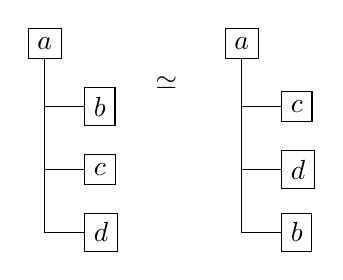
\begin{tikzpicture}[
                every node/.append style = {anchor = west},
                grow via three points={one child at (0.5,-0.8) and two children at (0.5,-0.8) and (0.5,-1.6)},
                edge from parent path={(\tikzparentnode\tikzparentanchor) |- (\tikzchildnode\tikzchildanchor)}]
            \node[draw] at (0,0) {\(a\)}
                child {node[draw] {\(b\)}}
                child {node[draw] {\(c\)}}
                child {node[draw] {\(d\)}};
            \node at (1.5,-0.5) {\(\simeq\)};
            \node[draw] at (2.5,0) {\(a\)}
                child {node[draw] {\(c\)}}
                child {node[draw] {\(d\)}}
                child {node[draw] {\(b\)}};
            \end{tikzpicture}
        \end{block}
    \end{minipage}
    ~\ ~\
    \begin{minipage}{0.45\textwidth}
        \begin{block}{}
            \[[a, b, c, d] \simeq [a, b, c, d]\]
            \centering
            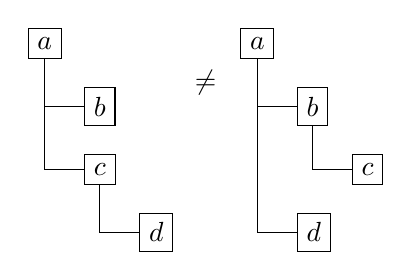
\begin{tikzpicture}[
                every node/.append style = {anchor = west},
                grow via three points={one child at (0.5,-0.8) and two children at (0.5,-0.8) and (0.5,-1.6)},
                edge from parent path={(\tikzparentnode\tikzparentanchor) |- (\tikzchildnode\tikzchildanchor)}]
                \node[draw] at (0,0) {\(a\)}
                    child {node[draw] {\(b\)}}
                    child {node[draw] {\(c\)}
                        child[draw] {node[draw] {\(d\)}}};
                \node at (2,-0.5) {\(\ne\)};
                \node[draw] at (2.7,0) {\(a\)}
                    child {node[draw] {\(b\)}
                        child {node[draw] {\(c\)}}}
                    child [missing] {}
                    child {node[draw] {\(d\)}};
            \end{tikzpicture}
        \end{block}
    \end{minipage}
\end{frame}

\begin{frame}[fragile]
    \frametitle{All strict child accesses are the same}
    \begin{minipage}{0.45\textwidth}
        \begin{block}{}
            {\tiny
            \begin{lstlisting}[language=rust, basicstyle=\ttfamily\scriptsize]
fn reborrow(x: &u64) -> &u64 {
    &*x
}
            \end{lstlisting}
            }
            {\small
            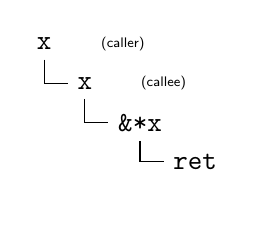
\begin{tikzpicture}[
                every node/.append style = {anchor = west},
                grow via three points={one child at (0.3,-0.5) and two children at (0.3,-0.5) and (0.3,-1.0)},
                edge from parent path={(\tikzparentnode\tikzparentanchor) |- (\tikzchildnode\tikzchildanchor)}]
            \node (nxcaller) at (0,0) {\texttt{x}}
                child {node (nxcallee) {\texttt{x}}
                    child {node {\texttt{\&*x}}
                        child {node {\texttt{ret}}
                            child {node {} edge from parent [draw=none]}}}};
            \node[right of=nxcaller] {\tiny(caller)};
            \node[right of=nxcallee] {\tiny(callee)};
            \end{tikzpicture}
            }
        \end{block}
    \end{minipage}
    ~\ ~\
    \begin{minipage}{0.45\textwidth}
        \begin{block}{}
            {\tiny
            \begin{lstlisting}[language=rust, basicstyle=\ttfamily\scriptsize]
fn reborrow(x: &u64) -> &u64 {
    &*&*x
}
            \end{lstlisting}
            }
            {\small
            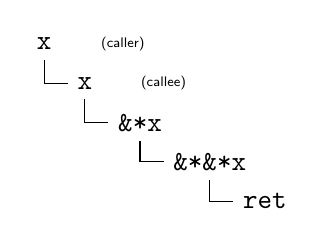
\begin{tikzpicture}[
                every node/.append style = {anchor = west},
                grow via three points={one child at (0.3,-0.5) and two children at (0.3,-0.5) and (0.3,-1.0)},
                edge from parent path={(\tikzparentnode\tikzparentanchor) |- (\tikzchildnode\tikzchildanchor)}]
            \node (nxcaller) at (0,0) {\texttt{x}}
                child {node (nxcallee) {\texttt{x}}
                    child {node {\texttt{\&*x}}
                        child {node {\texttt{\&*\&*x}}
                            child {node {\texttt{ret}}}}}};
            \node[right of=nxcaller] {\tiny(caller)};
            \node[right of=nxcallee] {\tiny(callee)};
            \end{tikzpicture}
            }
        \end{block}
    \end{minipage}

    \begin{block}{}
        {\small
            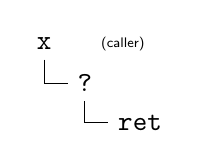
\begin{tikzpicture}[
                every node/.append style = {anchor = west},
                grow via three points={one child at (0.3,-0.5) and two children at (0.3,-0.5) and (0.3,-1.0)},
                edge from parent path={(\tikzparentnode\tikzparentanchor) |- (\tikzchildnode\tikzchildanchor)}]
            \node (nx) at (0,0) {\texttt{x}}
                    child {node {\texttt{?}}
                        child {node {\texttt{ret}}}};
            \node[right of=nx] {\tiny(caller)};
            \end{tikzpicture}
        }
    \end{block}
\end{frame}

\begin{frame}[fragile]
    \frametitle{All non-child accesses are the same}
        \begin{minipage}{0.28\textwidth}
        \begin{block}{}
            {\tiny
            \begin{lstlisting}[language=rust, basicstyle=\ttfamily\scriptsize]
let y = &*&*x;
x.do_something();
            \end{lstlisting}
            }
            {\small
                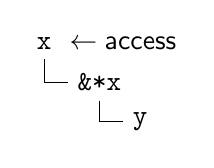
\begin{tikzpicture}[
                    every node/.append style = {anchor = west},
                    grow via three points={one child at (0.3,-0.5) and two children at (0.3,-0.5) and (0.3,-1.0)},
                    edge from parent path={(\tikzparentnode\tikzparentanchor) |- (\tikzchildnode\tikzchildanchor)}]
                \node (nx) at (0,0) {\texttt{x}}
                    child {node {\texttt{\&*x}}
                        child {node {\texttt{y}}}};
                \node[right of=nx] {\(\gets \text{access}\)};
                \end{tikzpicture}
            }
        \end{block}
    \end{minipage}
    ~\ ~\
    \begin{minipage}{0.28\textwidth}
        \begin{block}{}
            {\tiny
            \begin{lstlisting}[language=rust, basicstyle=\ttfamily\scriptsize]
let y = &*x;
x.do_something();
            \end{lstlisting}
            }
            {\small
                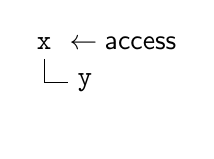
\begin{tikzpicture}[
                    every node/.append style = {anchor = west},
                    grow via three points={one child at (0.3,-0.5) and two children at (0.3,-0.5) and (0.3,-1.0)},
                    edge from parent path={(\tikzparentnode\tikzparentanchor) |- (\tikzchildnode\tikzchildanchor)}]
                \node (nx) at (0,0) {\texttt{x}}
                    child {node {\texttt{y}}
                        child {node {} edge from parent [draw=none]}};
                \node[right of=nx] {\(\gets \text{access}\)};
                \end{tikzpicture}
            }
        \end{block}
    \end{minipage}
    ~\ ~\
    \begin{minipage}{0.28\textwidth}
        \begin{block}{}
            {\tiny
            \begin{lstlisting}[language=rust, basicstyle=\ttfamily\scriptsize]
let y = &*x;
(&*x).do_something();
            \end{lstlisting}
            }
            {\small
                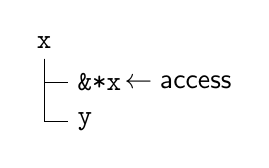
\begin{tikzpicture}[
                    every node/.append style = {anchor = west},
                    grow via three points={one child at (0.3,-0.5) and two children at (0.3,-0.5) and (0.3,-1.0)},
                    edge from parent path={(\tikzparentnode\tikzparentanchor) |- (\tikzchildnode\tikzchildanchor)}]
                \node (nx) at (0,0) {\texttt{x}}
                    child {node(nrefx) {\texttt{\&*x}}}
                    child {node {\texttt{y}}};
                \node[right of=nrefx] {\(\gets \text{access}\)};
                \end{tikzpicture}
            }
        \end{block}
    \end{minipage}


    \begin{block}{}
        {\small
            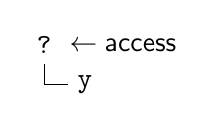
\begin{tikzpicture}[
                every node/.append style = {anchor = west},
                grow via three points={one child at (0.3,-0.5) and two children at (0.3,-0.5) and (0.3,-1.0)},
                edge from parent path={(\tikzparentnode\tikzparentanchor) |- (\tikzchildnode\tikzchildanchor)}]
            \node (nx) at (0,0) {\texttt{?}}
                    child {node {\texttt{y}}};
            \node[right of=nx] {\(\gets \text{access}\)};
            \end{tikzpicture}
        }
    \end{block}
\end{frame}

\begin{frame}
    \frametitle{One pointer, \(2 \times 2\) kinds of accesses}
    \begin{block}{}
        \centering
        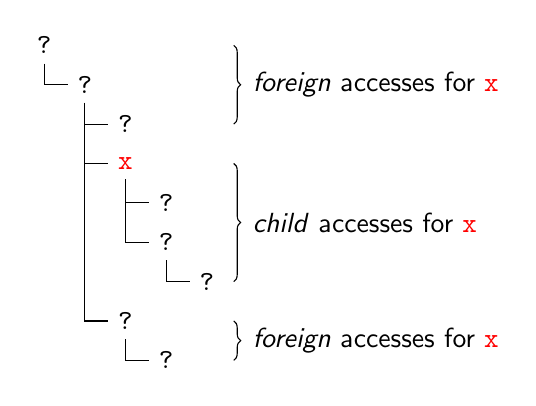
\begin{tikzpicture}[
            every node/.append style = {anchor = west},
            grow via three points={one child at (0.3,-0.5) and two children at (0.3,-0.5) and (0.3,-1.0)},
            edge from parent path={(\tikzparentnode\tikzparentanchor) |- (\tikzchildnode\tikzchildanchor)}]
            \node (root) at (0,0) {\texttt{?}}
                child {node {\texttt{?}}
                    child {node (nprevlast) {\texttt{?}}}
                    child {node (nxfirst) {\color{red}\texttt{x}}
                        child {node {\texttt{?}}}
                        child {node {\texttt{?}}
                            child {node (nxlast) {\texttt{?}}}}}
                    child[missing] {}
                    child[missing] {}
                    child[missing] {}
                    child {node (nnextfirst) {\texttt{?}}
                        child {node (nnextlast) {\texttt{?}}}}}
                ;
            \draw (2.5,0 |- root) node (vmark) {};
            \draw [decorate, decoration = {brace}] (vmark |- nxfirst) -- (vmark |- nxlast)
                node[midway] {~\textit{child} accesses for \color{red}\texttt{x}};
            \draw [decorate, decoration = {brace}] (vmark |- root) -- (vmark |- nprevlast)
                node[midway] {~\textit{foreign} accesses for \color{red}\texttt{x}};
            \draw [decorate, decoration = {brace}] (vmark |- nnextfirst) -- (vmark |- nnextlast)
                node[midway] {~\textit{foreign} accesses for \color{red}\texttt{x}};
        \end{tikzpicture}
        ~\\
        each \textit{read} or \textit{write}.
    \end{block}
    \begin{block}{Remark}
        Child accesses can be detected locally,
        so usually all unknown accesses are \textit{foreign} accesses.
    \end{block}
\end{frame}

\begin{frame}
    \frametitle{One tag, several pointers}
    \begin{block}{}
        \centering
        \begin{tikzpicture}[
            every node/.append style = {anchor = west},
            grow via three points={one child at (0.3,-0.5) and two children at (0.3,-0.5) and (0.3,-1.0)},
            edge from parent path={(\tikzparentnode\tikzparentanchor) |- (\tikzchildnode\tikzchildanchor)}]
        \node (nx1) at (0,0) {\texttt{x}}
                child {node {\texttt{y}}};
        \node (nx2) at (3,0) {\texttt{x}}
                child {node {\texttt{?}}
                    child {node {\texttt{y}}}};
        \node (nx2) at (6.5,0) {\texttt{x}}
                child {node {\texttt{?}}
                    child {node {\texttt{?}}
                        child {node {\texttt{y}}}}};
        \end{tikzpicture}
        ~\\
        \(\texttt{x} \to \texttt{y}\): foreign
        \(\qquad\)
        \(\texttt{y} \to \texttt{x}\): child;
    \end{block}
    \begin{block}{}
        \centering
        \begin{tikzpicture}[
            every node/.append style = {anchor = west},
            grow via three points={one child at (0.3,-0.5) and two children at (0.3,-0.5) and (0.3,-1.0)},
            edge from parent path={(\tikzparentnode\tikzparentanchor) |- (\tikzchildnode\tikzchildanchor)}]
        \node (nx1) at (0,0) {\texttt{x = y}};
        \node (nx2) at (3,0) {\texttt{x}}
                child {node {\texttt{y}}};
        \end{tikzpicture}
        ~\\
        \(\texttt{x} \to \texttt{y}\): child/foreign
        \(\qquad\)
        \(\texttt{y} \to \texttt{x}\): child;
    \end{block}
    \begin{block}{Later}
        This will be useful for raw pointers.
    \end{block}
\end{frame}

\begin{frame}
    \frametitle{Updates of permissions: general mechanics}
    \begin{block}{}
        \begin{align*}
                && \texttt{... | RW | RW | RW | ~~ | R~ | R~ | RW | ...} \\
              + && \texttt{~~~~~~~~~~<-~ foreign read ->~~~~~~~~~~~~~~~} \\
            \to && \texttt{... | RW | R~ | R~ | ~~ | R~ | R~ | RW | ...} \\
            UB: && \text{if the pointer is not allowed to lose write permissions}
        \end{align*}
    \end{block}
    \begin{block}{}
        \begin{align*}
                && \texttt{... | RW | RW | RW | ~~ | R~ | R~ | RW | ...} \\
              + && \texttt{~~~~~~~~~~<-~ child read ~~->~~~~~~~~~~~~~~~} \\
            \to && \texttt{... | RW | RW | RW | ~~ | R~ | R~ | RW | ...} \\
            UB: && \text{if the pointer does not currently have read permissions}
        \end{align*}
    \end{block}
\end{frame}



%\section{Deriving rules}

\begin{frame}[t]
    \frametitle{Active, Frozen, Disabled (very simplified)}
    Core triplet of permissions to represent
    \begin{itemize}
        \item unique mutable references: \texttt{Active},
        \item shared immutable references: \texttt{Frozen},
        \item lifetime ended: \texttt{Disabled}.
    \end{itemize}

    \begin{onlyenv}<1>
        \begin{block}{Child \textover{read}{write}: must allow reading}
            \begin{itemize}
                \item \texttt{Active} \(\to\) \texttt{Active}
                \item \texttt{Frozen} \(\to\) \texttt{Frozen}
                \item \texttt{Disabled} \(\to\) UB
            \end{itemize}
        \end{block}
        \includegraphics{steps.core.cr.pdf}
    \end{onlyenv}

    \begin{onlyenv}<2>
        \begin{block}{Child write: must allow writing}
            \begin{itemize}
                \item \texttt{Active} \(\to\) \texttt{Active}
                \item \texttt{Frozen} \(\to\) UB
                \item \texttt{Disabled} \(\to\) UB
            \end{itemize}
        \end{block}
        \includegraphics{steps.core.cr+cw.pdf}
    \end{onlyenv}

    \begin{onlyenv}<3>
        \begin{block}{Foreign \textover{read}{write}: no longer unique}
            \begin{itemize}
                \item \texttt{Active} \(\to\) \texttt{Frozen}
                \item \texttt{Frozen} \(\to\) \texttt{Frozen}
                \item \texttt{Disabled} \(\to\) \texttt{Disabled}
            \end{itemize}
        \end{block}
        \includegraphics{steps.core.cr+cw+fr.pdf}
    \end{onlyenv}

    \begin{onlyenv}<4>
        \begin{block}{Foreign write: no longer immutable}
            \begin{itemize}
                \item \texttt{Active} \(\to\) \texttt{Disabled}
                \item \texttt{Frozen} \(\to\) \texttt{Disabled}
                \item \texttt{Disabled} \(\to\) \texttt{Disabled}
            \end{itemize}
        \end{block}
        \includegraphics{steps.core.cr+cw+fr+fw.pdf}
    \end{onlyenv}
\end{frame}

\begin{frame}
    \frametitle{This simplified model already enforces}
    \begin{description}
        \item[\cmark] \texttt{Active} (\texttt{\&mut}) readable and writeable
        \item[\cmark] \texttt{Frozen} (\texttt{\&}) and all their children are only readable
        \item[\cmark] data behind \texttt{Active} (\texttt{\&mut}) is owned exclusively
        \item[\cmark] data behind \texttt{Frozen} (\texttt{\&}) is immutable
    \end{description}
\end{frame}


\section{Optimizations}

\begin{frame}
    \frametitle{Some standard optimizations}
    \begin{tabular}{|l|c|c|l}
        Possible in...                     & SB     & TB \\
        Insert speculative read            & \cmark & \cmark &\\
        Insert speculative write           & \cmark & \xmark &\visible<2>{\(\gets\)}\\
        Remove redundant read              & \cmark & \cmark &\\
        Remove redundant write             & \cmark & \cmark &\\
        Reorder read-write                 & \cmark & \xmark &\visible<2>{\(\gets\)}\\
        Reorder read-write (fn args)       & \cmark & \cmark &\\
        Reorder read-read                  & \xmark & \cmark &\visible<3>{\(\gets\)}\\
        Reorder read-read (fn args)        & \cmark & \cmark &\\
        Reorder write-write                & \cmark & \cmark &\\
        Reorder write-write (fn args)      & \cmark & \cmark &\\
        Reorder write-read                 & \cmark & \cmark &\\
        Reorder write-read (fn args)       & \cmark & \cmark &\\
        Reorder reborrow-reborrow          & \xmark & \cmark &\visible<3>{\(\gets\)}\\
    \end{tabular}
\end{frame}

\subsection{Possible optimizations}

\begin{frame}[fragile, t]
    \frametitle{{\cmark} Reorder write-any}
    \begin{onlyenv}<1>
        \begin{block}{}
            \begin{lstlisting}[language=rust, escapechar=@]
let x = &mut ...;
let y = &mut ...;
// x: Reserved
*x = 42; // (optimization: move down ?)
// x: Active
*y = 19; // is this a foreign write ?
// x: Active|Disabled -> UB

*x = 57;
// x: Active (Disabled -> UB)
            \end{lstlisting}
        \end{block}
    \end{onlyenv}
    \begin{onlyenv}<2>
        \begin{block}{}
            \begin{lstlisting}[language=rust, escapechar=@]
let x = &mut ...;
let y = &mut ...;
// x: Reserved


*y = 19; // assumed not to be a foreign write
// x: Reserved|Frozen|Disabled
*x = 42;
*x = 57;
// x: Active (Frozen|Disabled -> UB)
            \end{lstlisting}
        \end{block}
    \end{onlyenv}
    \begin{onlyenv}<3>
        \begin{block}{}
            \begin{lstlisting}[language=rust, escapechar=@]
let x = &mut ...;
// x: Reserved


*y = 19; // assumed not to be a foreign write
// x: Reserved|Frozen|Disabled

*x = 57;
// x: Active (Frozen|Disabled -> UB)
            \end{lstlisting}
        \end{block}
    \end{onlyenv}

\end{frame}

\begin{frame}[fragile, t]
    \frametitle{{\cmark} Insert speculative read}
    \begin{onlyenv}<1>
        \begin{block}{}
            \begin{lstlisting}[language=rust]
fn read(x: &u64) -> u64 {
    // x: [P] Frozen

    opaque(/* maybe foreign write */);
    // x: [P] Frozen (Disabled -> UB)
    *x // (optimization: move up ?)
}
            \end{lstlisting}
        \end{block}
    \end{onlyenv}

    \begin{onlyenv}<2>
        \begin{block}{}
            \begin{lstlisting}[language=rust]
fn read(x: &u64) -> u64 {
    // x: [P] Frozen
    let val = *x;
    opaque(/* assume no foreign write */);
    // x: [P] Frozen
    val
}
            \end{lstlisting}
        \end{block}
    \end{onlyenv}
\end{frame}

\subsection{Impossible optimizations}

\begin{frame}[fragile, t]
    \frametitle{Insert speculative write}

    \begin{exampleblock}{Possible strengthening}
        Write to mutable references on function entry.
    \end{exampleblock}

    \begin{onlyenv}<1>
        \begin{block}{{\xmark} Base model}
            \begin{lstlisting}[language=rust, basicstyle=\ttfamily\scriptsize]
fn foo(x: &mut u64) {
    // x: [P] Reserved

    opaque(/* maybe foreign read/write */);
    // x: [P] Reserved|Frozen (Disabled -> UB)
    *x = 42; // (optimization: move up ?)
}
            \end{lstlisting}
        \end{block}
    \end{onlyenv}

    \begin{onlyenv}<2>
        \begin{block}{{\cmark} Strengthened model}
            \begin{lstlisting}[language=rust, basicstyle=\ttfamily\scriptsize]
fn foo(x: &mut u64) {
    // x: [P] Active

    opaque(/* maybe foreign read/write */);
    // x: [P] Active (Frozen|Disabled -> UB)
    *x = 42;
}
            \end{lstlisting}
        \end{block}
    \end{onlyenv}

    \begin{onlyenv}<3>
        \begin{block}{{\cmark} Strengthened model}
            \begin{lstlisting}[language=rust, basicstyle=\ttfamily\scriptsize]
fn foo(x: &mut u64) {
    // x: [P] Active
    *x = 42;
    opaque(/* assume no foreign read/write */);
    // x: [P] Active (Frozen|Disabled -> UB)

}
            \end{lstlisting}
        \end{block}
    \end{onlyenv}

    \begin{onlyenv}<4>
        \begin{block}{{\cmark} ``\texttt{as\_mut\_ptr}'' pattern}
            \begin{lstlisting}[language=rust, basicstyle=\ttfamily\scriptsize]
// as_mut_ptr: &mut [T] -> *mut T (does not actually write)
let raw = buffer.as_mut_ptr(); // creates raw: Reserved
let shr = buffer.as_ptr().add(1); // creates shr: Frozen
                             // raw stays Reserved (foreign read)
copy_nonoverlapping(shr, raw, 1); // raw gets activated
            \end{lstlisting}
        \end{block}
    \end{onlyenv}

    \begin{onlyenv}<5>
        \begin{block}{{\xmark} ``\texttt{as\_mut\_ptr}'' pattern: strengthened model}
            \begin{lstlisting}[language=rust, basicstyle=\ttfamily\scriptsize]
// as_mut_ptr: &mut [T] -> *mut T (may speculatively write)
let raw = buffer.as_mut_ptr(); // creates raw: Active
let shr = buffer.as_ptr().add(1); // creates shr: Frozen
                             // raw becomes Frozen (foreign read)
copy_nonoverlapping(shr, raw, 1); // write through Frozen: UB
            \end{lstlisting}
        \end{block}
    \end{onlyenv}
\end{frame}

\begin{frame}[fragile, t]
    \frametitle{Reorder write-read}
%%% possible
    \begin{exampleblock}{Possible strengthening}
        Foreign read makes \texttt{Active} become \texttt{Disabled}
        (rather than \texttt{Frozen})
    \end{exampleblock}


    \begin{onlyenv}<1>
        \begin{block}{{\xmark} Base model}
            \begin{lstlisting}[language=rust, basicstyle=\ttfamily\scriptsize]
let x = &mut *y;
// x: Reserved
*x = 42; // (optimization: move down ?)
// x: Active
opaque(/* maybe foreign read/write */);
// x: Active|Frozen|Disabled


let _ = *x;
// x: Active|Frozen (Disabled -> UB)
            \end{lstlisting}
        \end{block}
    \end{onlyenv}

    \begin{onlyenv}<2>
        \begin{block}{{\cmark} Strengthened model}
            \begin{lstlisting}[language=rust, basicstyle=\ttfamily\scriptsize]
let x = &mut *y;
// x: Reserved
*x = 42; // (optimization: move down ?)
// x: Active
opaque(/* maybe foreign read/write */);
// x: Active|Disabled


let _ = *x;
// x: Active (Disabled -> UB)
            \end{lstlisting}
        \end{block}
    \end{onlyenv}

    \begin{onlyenv}<3>
        \begin{block}{{\cmark} Strengthened model}
            \begin{lstlisting}[language=rust, basicstyle=\ttfamily\scriptsize]
let x = &mut *y;
// x: Reserved


opaque(/* assume no foreign read/write */);
// x: Reserved
*x = 42;
// x: Active
let _ = *x;
// x: Active
            \end{lstlisting}
        \end{block}
    \end{onlyenv}

%%% impossible

    \begin{onlyenv}<4>
        \begin{block}{{\cmark} Reorder read-read}
            \begin{lstlisting}[language=rust]
let x = &mut *z; // x: Reserved
*x = 42; // x: Active
let _ = *x; // x: Active (optimization: move down ?)
let _ = *z; // x: Frozen (foreign read)

            \end{lstlisting}
        \end{block}
    \end{onlyenv}

    \begin{onlyenv}<5>
        \begin{block}{{\cmark} Reorder read-read}
            \begin{lstlisting}[language=rust]
let x = &mut *z; // x: Reserved
*x = 42; // x: Active

let _ = *z; // x: Frozen (foreign read)
let _ = *x; // x: Frozen
            \end{lstlisting}
        \end{block}
    \end{onlyenv}

    \begin{onlyenv}<6>
        \begin{block}{{\xmark} Reorder read-read: strengthened model}
            \begin{lstlisting}[language=rust]
let x = &mut *z; // x: Reserved
*x = 42; // x: Active
let _ = *x; // x: Active (optimization: move down ?)
let _ = *z; // x: Disabled (foreign read)

            \end{lstlisting}
        \end{block}
    \end{onlyenv}

    \begin{onlyenv}<7>
        \begin{block}{{\xmark} Reorder read-read: strengthened model}
            \begin{lstlisting}[language=rust]
let x = &mut *z; // x: Reserved
*x = 42; // x: Active

let _ = *z; // x: Disabled (foreign read)
let _ = *x; // Access through Disabled: UB!
            \end{lstlisting}
        \end{block}
    \end{onlyenv}
\end{frame}

\begin{frame}
    \frametitle{Summary}
    \begin{itemize}
        \item TB allows read reorderings (SB does not)
        \item TB allows speculative reads (SB as well)
        \item TB forbids speculative writes (SB allows them)
            \begin{itemize}
                \item the model can be strengthened to justify these optimizations...
                \item ...at the cost of common patterns.
            \end{itemize}
    \end{itemize}
\end{frame}


%\section{Evaluation}

\begin{frame}
    \frametitle{Counting crates with UB (1/2)}
    {\footnotesize
    Data obtained using \href{https://github.com/saethlin/miri-tools}{\texttt{github:saethlin/miri-tools}}\\
    }
    \begin{figure}
        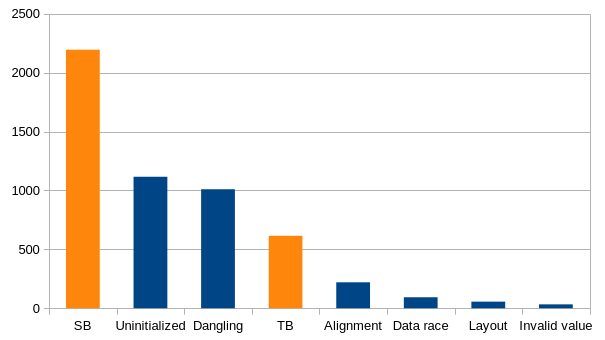
\includegraphics[width=0.8\textwidth]{../img/ub-count.png}
    \end{figure}
    {\footnotesize Number of crates on \texttt{crates.io} with at least one test
    that contains UB, for each kind of UB detected by Miri.}\\~\\
\end{frame}

\begin{frame}
    \frametitle{Counting crates with UB (2/2)}
    \begin{tabular}{|l|c|c|l|}
        \hline
        Kind                         &  SB &  TB & Notes\\
        \hline
        Protector invalidations      &  70 &  58 & \tiny(1) \\
        Protector deallocations      &  12 &  12 & \\
        Accesses without permissions & 998 & 545 & \tiny(2) \\
        Accesses outside range       & 903 &   0 & \tiny(3) \\
        Wildcard pointers            & 213 & --- & \tiny(4) \\
        \hline
    \end{tabular}
    Number of crates that contain UB, for subclasses of UB defined by SB and TB.~\\~\\
    From 97~851 crates, of which 3~808 contain UB of any kind\\~\\

    {\footnotesize
    \(^{(1)}\) now allowed: \texttt{Reserved -> Frozen}\\
    \(^{(2)}\) see: \texttt{as\_mut\_ptr}\\
    \(^{(3)}\) not included: accesses in wrong allocation\\
    \(^{(4)}\) not handled by TB\\
    }
\end{frame}

\begin{frame}
    \frametitle{Notable examples}
    \begin{block}{Accesses outside range}
        UB in \texttt{tokio}, \texttt{pyo3}, \texttt{rkyv}, \texttt{eyre}, \texttt{ndarray}, ...\\
        according to SB but not TB
    \end{block}
    \begin{block}{Invalidations by mutable reborrows (``\texttt{as\_mut\_ptr}'' pattern)}
        UB in \texttt{arrayvec}, \texttt{slotmap}, \texttt{nalgebra}, \texttt{json}, ...\\
        according to SB but not TB
    \end{block}
\end{frame}

\begin{frame}
    \frametitle{Summary}
    \begin{itemize}
        \item patterns allowed by Stacked Borrows but forbidden by Tree Borrows are rare
        \item Tree Borrows UB is much less common on \texttt{crates.io}
        \item elimination of out-of-bounds UB
    \end{itemize}
\end{frame}

\begin{frame}
    \frametitle{Questions ?}

    TB also has...
    \begin{itemize}
        \item tweaked rules for interactions between interior mutability and protectors/\texttt{Reserved}
        \item performance improvements compared to the naive implementation
            \begin{itemize}
                \item many tricks to trim tree traversals
                \item lazy initialization for out-of-range accesses
            \end{itemize}
        \item ongoing attempt at formalization in Coq
    \end{itemize}
\end{frame}


\end{document}
